\chapter{MorpheesPlugs}
  \begin{figure}[h]
    \centering
    \subfloat[]{
      \label{fig:animal_family}
      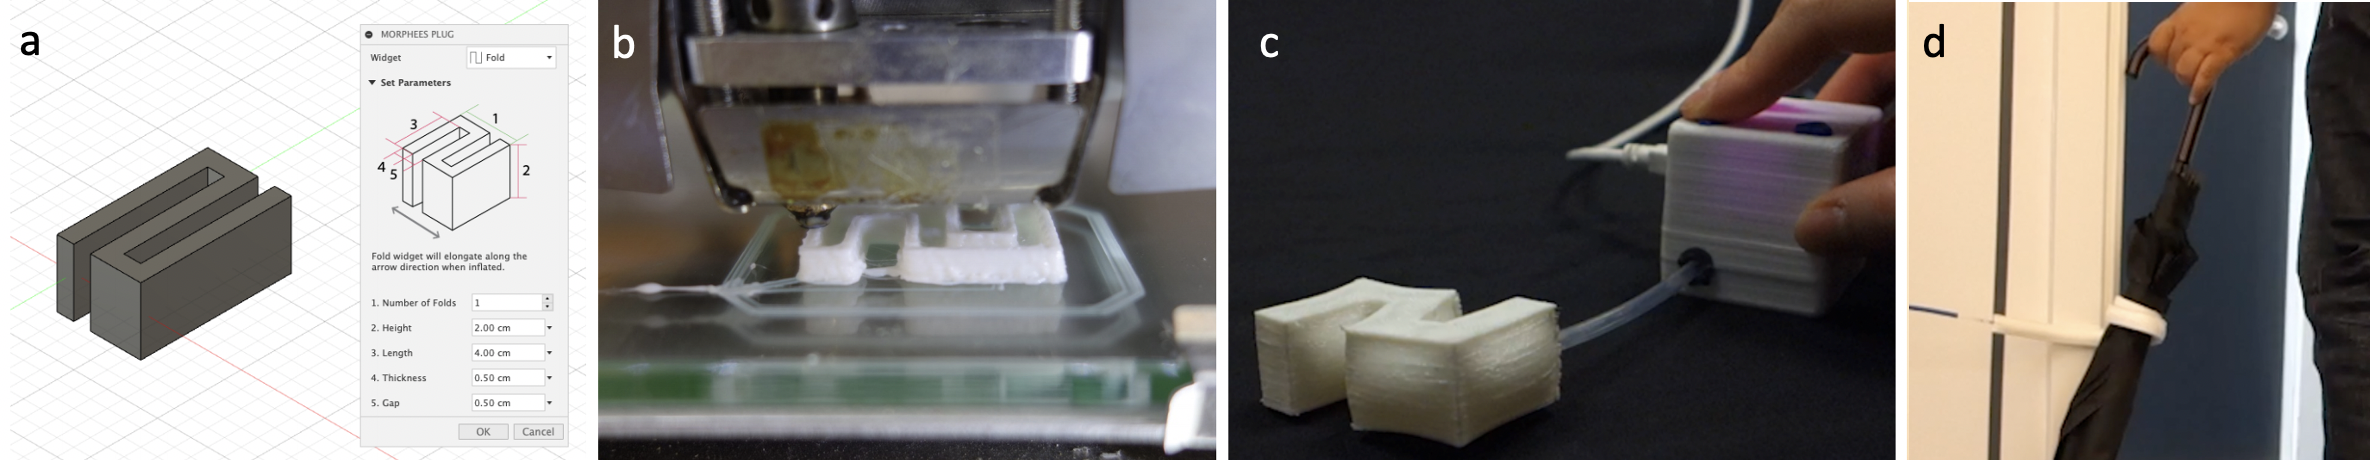
\includegraphics[width=0.33\textwidth]{print-and-play/morphees/Fig_1.png}
    }
    \label{fig:teaser}

    \caption{\mp is a toolkit to prototype shape-changing interfaces. (a) Users
      first use software to design a \textit{widget} that can express
      shape-change, such as length or curvature change. (b) They then 3D print the
      widget with an off-the-shelf 3D printer. (c) They plug the widget into a
      control module that can adjust air pressure in the widget and actuate the
      widget. (d) An example application. The printed shape-changing interface
      holds the umbrella and gently pushes the umbrella towards user so that users
      can be reminded to take the umbrella.}
  \end{figure}

  \section{Abstract}
    Toolkits for shape-changing interfaces (SCIs) enable designers and researchers
    to easily explore the broad design space of SCIs. However, despite their
    utility, existing approaches are often limited in the number of shape-change
    features they can express. This paper introduces \mp, a toolkit for creating
    SCIs that covers seven of the eleven shape-change features identified in the
    literature. \mp is comprised of (1) a set of six standardized widgets that
    express the shape-change features with user-definable parameters; (2) software
    for 3D-modeling the widgets to create 3D-printable pneumatic SCIs; and (3) a
    hardware platform to control the widgets. To evaluate \mp we carried out ten
    open-ended interviews with novice and expert designers who were asked to
    design a SCI using our software. Participants highlighted the ease of use and
    expressivity of the MorpheesPlug.

  \section{Introduction}
    Shape-Changing Interfaces (SCIs) are emerging as a new generation of
    devices that can change their shapes to support dynamic affordances
    \cite{10.1145/2501988.2502032}, leverage human dexterity \cite{6926382},
    and support the personalization of physical interfaces
    \cite{10.1145/1357054.1357090}. The current design space of SCIs covers a
    wide range of features \cite{10.1145/3173574.3174193}, including variable
    length \cite{10.1145/2501988.2502032}, volume
    \cite{10.1145/1357054.1357090}, curvature \cite{Yao:2013bg}, and porosity
    \cite{10.1145/1517664.1517671}. The literature has featured numerous
    prototype systems exploring a huge variety of shapes, shape-changes,
    interactions, implementation techniques, and applications. 
    
    Despite the potential of SCIs to enhance the development of the
    next generation of interactive devices, there are still many challenges
    faced by the field \cite{10.1145/3173574.3173873}. One major barrier to
    the creation of SCIs is the lack of standardized toolkits for
    exploration and development \cite{10.1145/3173574.3173873}. Current
    approaches require substantial time, effort, domain-specific knowledge,
    and complex tools to create even simple SCIs. Unlike software-only
    user interfaces, physical UIs---including SCIs---interact with
    physical reality, requiring the addition of hardware components.
    Researchers have developed physical toolkits to simplify creating physical
    UIs, providing standardized hardware widget libraries
    \cite{Greenberg:2001,Bdeir:2009kz} and tools to ease the communication
    between the digital and physical worlds \cite{Hartmann:2007p4338}.
    
    Shape-Changing Interfaces introduce new problems, because there are no
    standardized widget libraries, actuation methods, or design tools. It
    means that to experiment with or develop such UIs requires users need to
    design, fabricate, and implement all aspects of shape-changing systems. As
    a result, the literature illustrates many one-off application-specific
    SCIs \cite{Sturdee:2018ce}. Alexander \etal note that a primary necessary
    strand of the field is to create ``a standard platform for hardware
    prototyping''.
    
    There are two primary challenges to creating such a standardized toolkit
    for prototyping SCIs. The first is \textit{actuation}: given a
    desired shape change, how to choose a technical method to cause that
    transformation. Researchers have identified dozens of shape-change
    features \cite{10.1145/3173574.3174193} (e.g., length) and actuation
    methods \cite{Sturdee:2018ce} (e.g., servo motor), but there are no
    standards or guidelines for how a user can select a method to implement a
    desired feature.
    
    Closely coupled with the issue of actuation is that of
    \textit{fabrication}: how to physically instantiate an actuation method
    that causes the desired shape-change. Toolkits for physical UIs offer
    pre-made physical widgets that let users concentrate on applications
    \cite{Greenberg:2001,Bdeir:2009kz}, but the bulk of the SCI literature
    focuses on novel techniques (e.g., \cite{10.1145/2984511.2984520}) or
    applications rather than broadly reusable widgets. The result is that SCIs
    tend to be one-offs, custom-made for a specific application, and require
    extensive technical prototyping skills.
  
    As a first step towards addressing these challenges, we introduce \mp, a
    toolkit aimed at simplifying the design, fabrication, and actuation of
    SCIs. \mp does so by following in the footsteps of successful GUI
    and physical computing toolkits: providing physical widgets, control
    hardware and firmware, and a design environment. \mp simultaneously
    addresses the \textit{actuation} and \textit{fabrication} challenges by
    providing six pneumatically powered shape-changing widgets which express a
    broad range of shape-change features from the Morphees+ framework
    \cite{10.1145/3173574.3174193}. Users can customize these widgets and
    incorporate them in their own SCI designs, eliminating the need to choose
    an actuation method for specific shape-change features and simplifing the
    design process. \mp widgets are printable on commodity 3D printers with
    standard flexible filament, significantly lowering the barrier to
    prototyping SCIs. 

    With \mp, we make the following contributions:     
      \begin{enumerate}
        \item We provide six customizable, 3D-printable widgets that express
          a wide range of shape changes via pneumatic actuation.
        \item We characterize widget performance over a variety of printing
          parameters, illustrating the range of shape changes available.
        \item We implement and publicly share design software and control
          module for the
          widgets~\footnote{\url{https://github.com/shape-changing-interfaces/MorpheesPlug}}.
        \item We demonstrate the utility of our toolkit via five
          proof-of-concept applications and a qualitative user study.
      \end{enumerate}

  \section{Related Work}
    \mp is a toolkit that simplifies creating and exploring SCIs, using
    pneumatic widgets. As such, it is situated at the intersection of
    SCIs, physical UI toolkits, and pneumatically actuated soft UIs and
    robotics. In this section, we situate \mp in the context of toolkit
    research, both for SCIs and physical UIs. Then we look into how
    pneumatic actuation was used for shape-changes.
    
    \subsection{Toolkits for Shape-Changing Interfaces}
      Alexander \etal \cite{10.1145/3173574.3173873} identified twelve grand
      challenges in SCIs research. Although many types of SCIs have been
      explored in the literature \cite{Sturdee:2018ce}, most are custom-made,
      one-off projects developed to illustrate an interaction technique,
      actuator, or application; hence, Alexander \etal
      \cite{10.1145/3173574.3173873} call for the development of
      \textit{toolkits for SCI} to ``dramatically lower the barrier to
      implementation''. They call for three advances in research: a hardware
      prototyping platform, a software application layer, and tools for end-user
      programming. To these three we add a fourth important need, adapted from
      Ledo \etal \cite{10.1145/3173574.3173610}: empowering new audiences,
      implying ease of acquisition or fabrication. A number of projects in the
      literature aim to overcome these barriers, either by explicitly presenting
      toolkits for SCIs or by addressing one or more of these challenges.
      
      Ledo \etal \cite{10.1145/3173574.3173610} define toolkits as
      ``present[ing] users with a programming or configuration environment
      consisting of many defined permutable building blocks, structures, or
      primitives, with a sequencing of logical or design flow affording a path
      of least resistance''. While few papers in the SCI space explicitly
      identify their work as presenting toolkits, in this section we include
      research which addresses any aspects which could be useful as part of a
      toolkit.
      
      Perhaps the most comprehensive example of a SCI toolkit is ShapeClip
      \cite{Hardy:2015dx}, a set of 1D linear actuators controlled by light
      emitted from standard computer screens. While it addresses Alexander
      \etal's three research threads, the ShapeClip hardware consists of complex
      electromechanical components not readily accessible to casual users. The
      hardware also limits the types of shape-change to those that can be
      expressed via length feature.
      
      Other systems, while not explicitly identified as toolkit research,
      present useful hardware building blocks for SCIs. One approach is to use
      electromechanical actuators as a driver of shape-change; for example,
      perhaps the earliest example approaching an SCI toolkit was Topobo
      \cite{Raffle:2004jj}, a system of passive and active (motorized) building
      blocks that could record and re-play movements. LineFORM
      \cite{10.1145/2807442.2807452} and ChainFORM \cite{nakagaki2016chainform}
      are similarly collections of actuators which can record and re-play
      movements, but focus on rotational rather than linear motion. Each of
      these systems is constrained by its actuators: using motors limits the
      minimum size, dictates the kinds of shape-change transformations
      available, and leads to high-complexity hardware, requiring custom
      circuitry that is unavailable to a casual user.
      
      Another type of SCI system uses shape-memory alloys or nitinol wires to
      actuate shape changes. shape-memory alloy-based actuation has the
      advantage of small size and flexibility, but at the expense of actuation
      speed. One early example, Bosu \cite{10.1145/1858171.1858205}, offered a
      set of frames and fabric shapes on which the shape-memory alloy wires
      could be fixed. While these components formed a small library of
      transformable shapes, Bosu required users to assemble each component
      manually.  NURBSforms \cite{10.1145/3374920.3374927} operated on the same
      principle as Bosu, but used flexible circuit boards, providing a
      standardized---and potentially mass-manufacturable---format. Both of these
      toolkits demonstrate shape changes based primarily on the curvature
      feature from Morphees+ \cite{10.1145/3173574.3174193}, a result of the
      low-amplitude length change possible with shape-memory alloys.
      
      Some systems use pneumatic actuation to transform shapes. One of the
      earliest projects in this space was PneUI \cite{Yao:2013bg}, which offered
      a technological framework for pneumatically actuated shape-change.
      Although the downside was that its shape-changing objects were all
      manually created, it illustrated the versatility of soft, pneumatic
      shape-change via multiple types of transformations, including curvature,
      volume, and texture. Other pneumatically actuated SCIs include
      Printflatables \cite{10.1145/3025453.3025898} and AeroMorph
      \cite{10.1145/2984511.2984520}, both of which require custom-built
      equipment to create, and Siloseam \cite{10.1145/3357236.3395473}, which
      presents a manual workflow for shape-changing silicone bladders.
      
      Aside from ShapeClip, none of these examples present themselves as toolkit
      research. Instead, they focus more on novel actuation schemes and
      possibilities for expressing shape changes. One result of this limited
      focus is the lack of standardized widgets to express a wide range of
      shape-change features: most of these systems present at most one or two
      reusable transforming shapes and can express a fraction of the Morphees+
      \cite{10.1145/3173574.3174193} feature space. Our goal with \mp is to
      provide a diverse set of shape-change widgets that enable experimentation
      with much larger coverage of the feature space, while being easily
      fabricated by users with minimal required equipment and expertise.
        
    \subsection{Physical UI Toolkits}
      Although few toolkits exist for SCIs, many of the same challenges are
      addressed by toolkits for physical user interfaces; in fact, SCIs can be
      viewed as a subset of physical UIs. In contrast to GUIs which take
      advantage of standardized hardware such as touchscreens or keyboards,
      physical UI toolkits aim to make novel input and output mechanisms
      accessible to non-expert users.
      
      One of the earliest physical computing toolkits was Phidgets
      \cite{Greenberg:2001}. It applied the idea of GUI widgets to physical
      interaction controls, enabling a combination of function and interface in
      a reusable building-block component. Later physical UI toolkits expanded
      on this idea, adding novel connections between modules
      \cite{Bdeir:2009kz}, more powerful widgets \cite{Villar:2012hd}, or novel
      form-factors \cite{Hodges:2014}. These examples illustrate a
      \textit{prefabricated} approach, where the physical widgets are designed
      and manufactured by a third party, and end users assemble, but don't
      usually modify them. The advantage of this approach is less work for
      users, who can experiment with a set of validated widgets. The downside is
      that form-factors and capabilities are limited by the widget
      manufacturer's priorities.
      
      A second approach to physical widgets is custom-fabrication. Toolkits in
      this category provide assistance to users in creating widgets (or
      widget-like components) tailored for a particular application. Midas
      \cite{Savage:2012ev}, for example, provided tools to help users fabricate
      customized touch sensors that could wrap around objects of varying sizes;
      Pineal \cite{Ledo:2017ks} added ``remote widgets'' to smartphones and
      watches via automated 3D modeling; and PaperPulse \cite{Ramakers:2015gi}
      fabricated predefined widgets with conductive inkjet printing. The
      advantage of this approach is much-greater flexibility: users can include
      different sizes and types of widgets in many configurations. However,
      customized widgets for each application can mean much greater time and
      effort for the user.
      
      \mp takes inspiration from both types of physical computing toolkit. We
      provide a set of predefined shape-change widgets which are customizable in
      the design stage, and then can be fabricated on unmodified commodity 3D
      printers. In this way we aim to support users with a set of pre-validated
      widgets that can be re-used if desired, but that have enough
      customizability to be tailored for a variety of applications.
        
    \subsection{Pneumatic Shape-Change}
      In order to grant \mp widgets the broadest range of possible shape
      changes, while still being easily fabricatable by end users, we use air
      pressure as an actuation source. Many other projects in HCI and other
      fields have similarly used pneumatics for driving flexible interfaces and
      robotics.

      Examples of pneumatically driven interfaces have mainly concentrated on
      exploring the diversity of interaction that such soft interfaces can
      offer. For example, Kim \etal's Inflatable Mouse \cite{Kim:2008du}
      illustrated multiple input and output behaviors, Harrison and Hudson's
      inflatable buttons provided dynamic haptics \cite{Harrison:2009}, and
      PneUI \cite{Yao:2013bg} demonstrated a wide variety of shape changes
      possible with elastic air bags. Despite the versatility of these
      interfaces, they are difficult to create, involving intensive manual
      assembly. Recent work by Moradi and Torres \cite{Moradi:2020} underscores
      both the versatility and difficulty of working with flexible materials,
      demonstrating a wide range of shape change and investing considerable
      effort in laying out a workflow to lessen the effort of fabrication.

      Some research has investigated 3D printing for pneumatically actuated
      SCIs. Although subject to the limitations of 3D printers, creating SCIs
      this way can---at least in theory---significantly lessen the effort
      required to create usable transforming objects. Vazquez \etal created a
      series of physical widgets using 3D printing \cite{Vazquez:2015dm}, and
      Lee \etal developed a system of Lego-compatible pneumatic blocks for
      experimenting with soft robotics \cite{Lee:2018}. These projects relied on
      high-end multi-material inkjet-based 3D printers, which are not currently
      easily accessible to most end users; the materials available for these
      printers have low stretchability. Another possibility for 3D printing
      flexible objects is via FDM printing, using flexible filaments such as
      thermoplastic polyurethane (TPU). Thus far, most progress in TPU actuators
      has been made in the field of soft robotics, where the emphasis has been
      on locomotion and grasping \cite{Yap:2016}.
      
      \mp's pneumatic actuation is inspired by these previous efforts. Despite
      the versatility of these related approaches, their main shortcoming is
      ease of use, requiring complex fabrication, and actuation techniques. We
      directly tackle these challenges in two ways. First, we provide users with
      an easy-to-use design environment for creating SCIs. Second, \mp uses
      inexpensive off-the-shelf fabrication equipment and material to create
      multiple widgets, enabling a wide range of shape-change possibilities.

  \section{Design Rationale} 
    Before building \mp, a toolkit for prototyping SCIs, we discuss what
    kind of design goals we wanted to achieve in \mp in terms of toolkit design.
    We looked into review literature that suggests design guidelines for
    toolkits \cite{10.1145/3173574.3173610}. Here we discuss how \mp meets four
    of the five goals in toolkit research.
      
    \begin{enumerate}
      \item \textit{Reducing Authoring Time and Complexity.}
        Fabricating SCIs is a challenging task. This process often entails the
        use of specialized equipment and requires engineering expertise. To
        address this challenge, we encapsulate the knowledge of the type of
        shape-change our six widgets will exhibit when pneumatically actuated.
        This, coupled with the analysis of how each widget implements features
        of SCIs taxonomies, allows designers to have an estimation of the
        expected shape-change the widgets will exhibit before fabricating them,
        reducing time, effort, and domain knowledge when building new SCIs.
        
      \item \textit{Empowering New Audiences.}
        Complex 3D modeling and electrical engineering can be a barrier for
        non-expert users who want to step in the area of SCIs. To simplify the
        process of designing the widgets \cite{Olsen:2007ik}, we provide a
        plug-in for CAD software that is widely available. Without a need for
        manually 3D modeling the widgets, users can choose the widget type and
        alter the parameters of it to to create 3D models with the plug-in. To
        evaluate if \mp can be used by new audience than researchers in SCI
        field, we conduct a user study with hobby makers.
        
      \item \textit{Integrating with Current Practices and Infrastructures.}
        While pneumatically actuating SCIs allows designers to create a wide
        range of shape-change with a single actuation method, the fabrication of
        these artifacts is not always a straightforward process, often requiring
        manual assembly~\cite{Yao:2013bg}, or special
        machinery~\cite{10.1145/3025453.3025898, 10.1145/2984511.2984520}. Our
        work aims to use existing, consumer-level tools (e.g., off-the-shelf
        3D-printers, materials, and design tools) to fabricate SCIs.
        
      \item \textit{Enabling Replication and Creative Exploration.}
        Ideal toolkits should support easy replication of previous work
        \cite{Greenberg2007} and exploring design spaces that has not examined
        before \cite{Olsen:2007ik}. To show that \mp has such properties, we
        replicate one of the SCIs that had a huge impact in the field
        \cite{10.1145/2501988.2502032} as well as suggest novel interfaces with
        \mp.
    \end{enumerate}
          
    Based on these design goals, we designed \mp. We aimed to build \mp to be
    easy to use for researchers as well as engineering novices to significantly
    reduce their iteration time and effort. One goal suggested for toolkit
    design that we did not aim was \textit{Creating Paths of Least Resistance,}
    which means that toolkits should guide users to design good interfaces
    rather than bad ones \cite{Myers:2000us, 10.1145/3173574.3173873}.
    SCI field is still at the early stage, and we believe that there are
    too few design guidelines to be generalized (e.g.,
    \cite{10.1145/2556288.2557360, 10.3389/frobt.2019.00079,
    10.1145/2858036.2858350}) comparing to the vast design space of SCIs.
    Therefore, we planned not to guide users what kind of SCIs they should
    design at this stage of the research.  Future studies can contribute to the
    design guidelines for SCIs using \mp, as it would allow quickly implementing
    a wide range of SCIs.

  \section{\mp Widgets}
    \mp is comprised of three basic components: (1) a set of shape-changing
    widgets; (2) a design environment; (3) a control module. A widget is the
    minimum unit in \mp that creates shape-change when 3D-printed and then
    pneumatically actuated. Widgets are the core of \mp. The design interface is
    a plug-in for CAD software that users can create 3D models of the widgets
    and customize them on the software. A module is a physical interface that
    users can control air pressure in a widget. This section shows how we
    designed the widgets and how they can express shape-change features.
      
    We designed the widgets primarily based on the features and also literature
    from HCI, soft robotics, and material science. Note that we excluded the
    speed, feature, because the feature relies on the actuation method, not the
    design of the widgets. Also, we did not include stretchability, granularity,
    and strength, because we first wanted to focus on features that involve
    clear visual shape-changes in the scope of the paper.
    Figure~\ref{fig:widget_all} shows the widgets we designed, and
    Figure~\ref{fig:widget_all_table} shows how the widgets can express
    shape-change features. Below, we describe how we designed each widget and
    how they can express the shape-change features.
      
    \begin{figure}[htb]
      \centering
      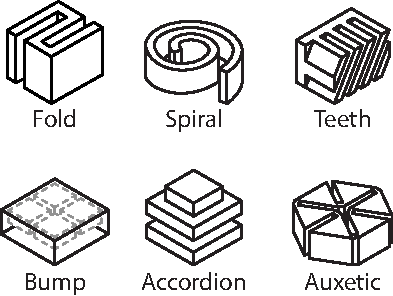
\includegraphics[width=0.3\textwidth]{print-and-play/morphees/Widget_all.pdf}
      \caption{The six widgets that \mp provide. The widgets can express
        different shape-change features such as length, curvature, etc.}
      \label{fig:widget_all}
    \end{figure}
        
    \begin{figure*}[htb]
      \centering
      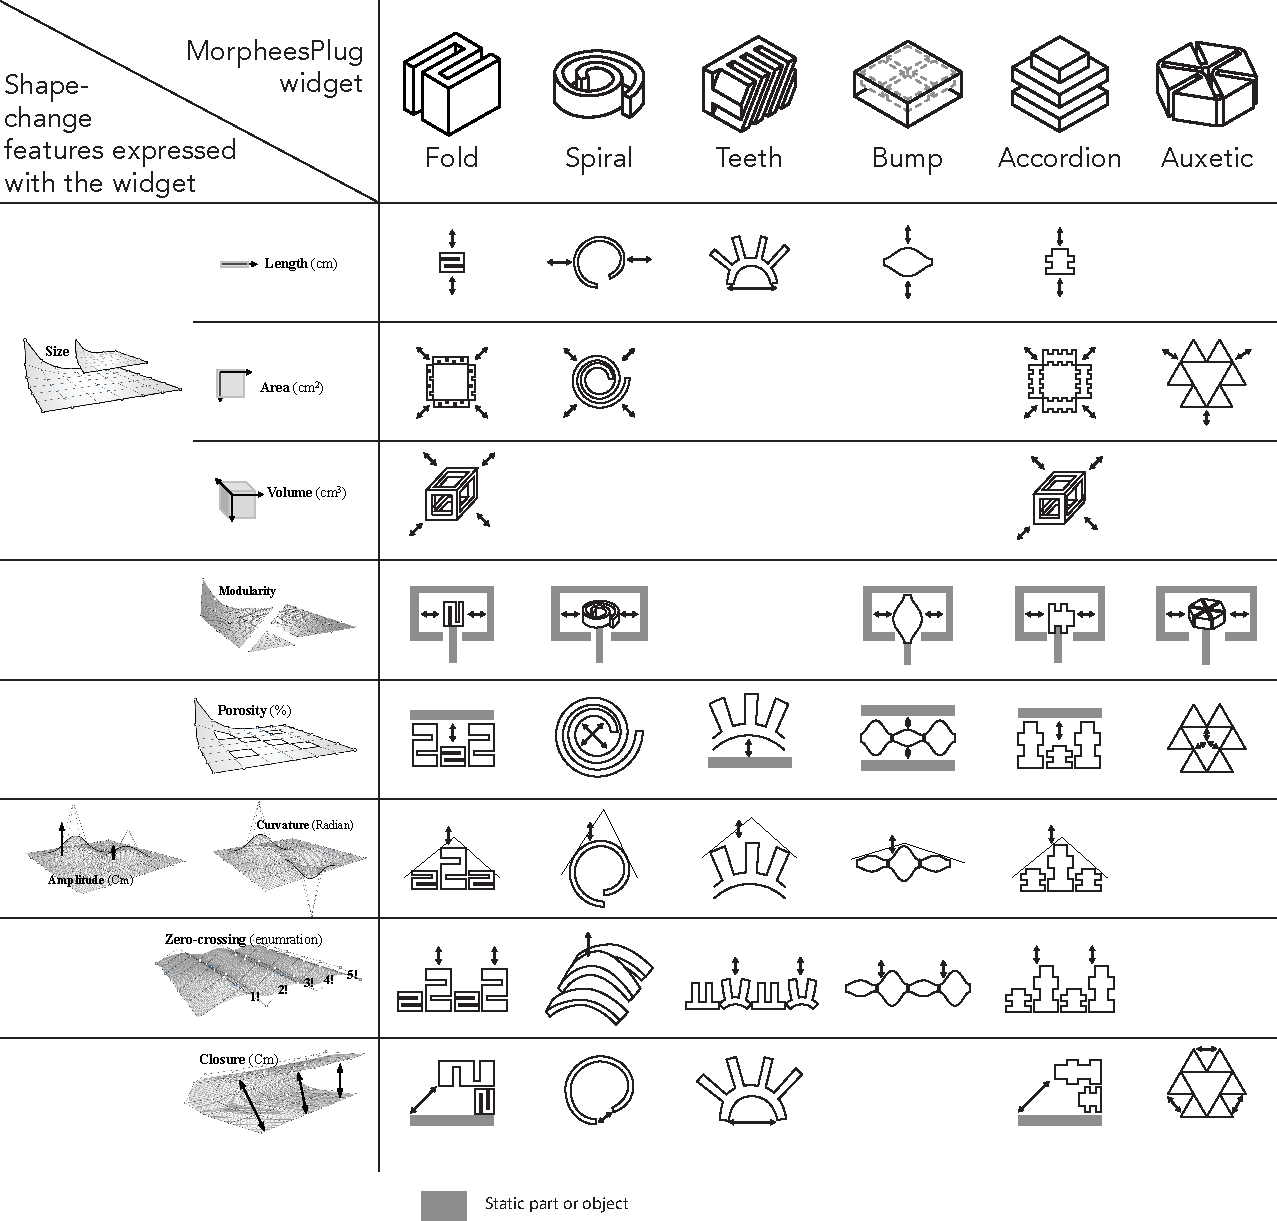
\includegraphics[width=\textwidth]{print-and-play/morphees/Table1_widgets_featuresv8.pdf}
      \caption{Top: Widgets provided by MorpheesPlug. Left: shape-change
        features from literature \cite{Roudaut:2013kz, 10.1145/3173574.3174193}.
        Middle: Illustrations of how the widgets can express the shape-change
        features.}
      \label{fig:widget_all_table}
    \end{figure*}
    
    \subsection{Fold widget}
      The Fold widget is a widget that is primarily designed to implement
      length change ( Figure~\ref{fig:widget_all_table}).  It is consists of a
      single layer of thin chamber that is folded in 90 degrees several times.
      The structure was originally used in material science \cite{Carpi_2007}
      as a dielectric elastomer actuator. When inflated, the fold slightly
      opens, and the whole structure elongates.
        
      We found that the widget can implement all of the shape-change features
      we aimed for. For example, when length-changing widgets are connected to
      make a rectangular shape or cube, they can also implement area and
      volume features under the size feature.  To change modularity feature,
      it can be attached a a static object and elongate in a slot. It would
      lock the static object and slot together.  To express porosity, there
      can be several Fold widgets and a solid surface on top of them. When the
      widgets elongate, they close the space between the widgets and the
      surface. When they shorten, they open the space and increase porosity.
      We considered that the widget can express amplitude and curvature
      features at the same time. When there are multiple Fold widgets on the
      same flat surface and some of them elongate, the surface would look like
      a curved surface. It would express amplitude and curvature features.  In
      the same sense, when the widgets elongate while some in between them do
      not, they can express zero-crossing.  Lastly, when the widget is placed
      aligned to a surface and elongates, it would change closure feature
      between an end of the widget and an end of the surface.
        
    \subsection{Spiral widget}
      Spiral widget is a widget that has a curved thin chamber. When looked
      from the top of the widget, it resembles a spiral shape. This widget is
      design to express changes in the curvature feature. When inflated, the
      curved surface unbends and changes the angle between the central point
      and the end points of the surface. This widget can also represent
      changes in the length feature. When inflated, the distance between two
      diametrically opposed point increases. Additionally, if the widget is
      designed to have multiple arcs, its enveloping area increases when
      inflated. While doing so, the porosity of the widget also increases as
      the space between the arcs increases.  Similarly to Fold widgets, a
      Spiral widget can be put in a slot and inflated to lock itself in the
      slot. In this way, the two objects that contain the slot and the widget
      can combine into one and change modularity feature.  When a Spiral
      widget changes curvature, it also changes amplitude.  The widget can
      also express zero-crossing. When there are multiple Spiral widgets
      placed next to each other and when only some of them are deflated, the
      deflated widgets would create bumpy surfaces therefore change
      zero-crossing.  When a Spiral widget has a single spiral and is
      inflated, the distance between the two end points increases, changing
      closure.
        
    \subsection{Teeth widget}
      Similarly to the Spiral widget, Teeth widget is designed to express
      curvature and amplitude. However, unlikely to Spiral, a Teeth widget has
      a straight shape when deflated and bends when inflated.  The length
      between two end points of a Teeth widget would be decreased when the
      widget is inflated.  Users can put a Teeth widget on a flat surface and
      increase porosity between the widget and the surface by inflating the
      widget.  By connecting multiple Teeth widgets and inflating one of every
      second of them, users can express zero-crossing.  When it is inflated
      the two ends of the widget get closer, expressing closure feature.
        
    \subsection{Bump widget}
      Bump widget is designed to have it on a flat surface and express a bumpy
      surface on it.  Users can have several of them connected to each other.
      When one Bump widget is inflated, it can express the length feature.
      When it is inflated in a slot, it can lock an object attached it and the
      slot, expressing modularity.  When there are multiple Bump widgets and
      there are static objects on and under them, inflation of the widgets
      would change porosity between the widgets and the objects.  Similarly,
      when there are multiple Bump widgets and only some of them are inflated,
      they change amplitude, curvature, and zero-crossing.
        
    \subsection{Accordion widget}
      Accordion widget is designed to take advantages of both Fold and Bump
      widgets. Like the Fold widget, it can express length feature when
      elongated. Thanks to it, it can express all the features that Fold
      widget can express.  Like Bump widget, it can have several chambers on
      the surface like tiles.  Because the chambers are connected, users can
      express curvature, amplitude, and zero-crossing features on a connected
      smooth surface, similarly to PolySurface \cite{everitt2017polysurface}.
      Thanks to the grooved surfaces on the four sides, it can have more
      length change than Bump widget.
        
    \subsection{Auxetic widget}
      We designed our auxetic widget to display porosity feature. I got
      inspired from the literature \cite{grima2006auxetic}. When inflated, the
      widget opens up width-wise, enlarging a central area and thus increasing
      its porosity. In addition, once actuated, the width of this widget
      increases, also displaying shape-change in the area feature. Further,
      when it has reach its maximum shape-change, the outer shapes of separate
      from each other, exhibiting the closure feature. Lastly, it is able
      display the modularity feature once expanded by attaching to near
      objects.

  \section{Implementation}
    \mp is comprised of three main components: (1) a set of 3D-printable,
    inflatable widgets that can represent seven out of eleven of the Morphees+
    features ~\cite{10.1145/3173574.3174193}; (2) a design environment for
    makers to model SCIs; (3) a control module responsible for actuating SCIs
    widgets. All of the resulting output (hardware, firmware, software, and
    designs) will be made available online under the MIT license.

    \subsection{Design Software}
      Our design environment is built on top of Autodesk Fusion 360 (Figure
      \ref{fig:plugin}) using its Python API for scripting remote command
      execution. In order to design a shape-changing widget using our tool, the
      user selects the desired widget from a drop-down list, and proceeds to
      modify the controlling parameters. The design automatically updates to
      match the user's inputs.
      
      \begin{figure}[htb]
        \centering
        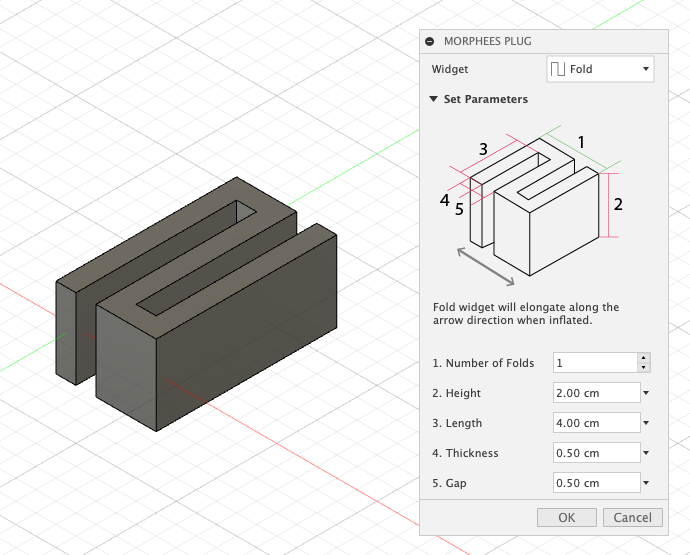
\includegraphics[width=0.45\textwidth]{print-and-play/morphees/Teasure_plugin.png}
        \caption{Detail view of our design environment, based on Autodesk Fusion
          360. The user is presented with a window where they can specify the
          sizes for the different parameters that compose our widgets.}
        \label{fig:plugin}
      \end{figure}

    \subsection{Fabrication}
      All \mp widget designs are printed as a single structure using
      consumer-grade FDM~\footnote{Fused Deposition Modeling} 3D-printers with
      elastic filament (NinjaFlex, shore 85A). To test our designs, we
      fabricated dozens of our widgets using three different 3D-printers
      (Lulzbot Taz 6, Ultimaker 2, and Crealitly Ender 3 Pro). During our
      initial tests, we found that the default print settings for these printers
      would produce non-airtight objects, causing the resulting objects to
      exhibit very little shape-change, if at all. To address this, we explored
      different printing settings for each of our printers, and got best results
      by over-extruding our designs, lowering the print speed, and increasing
      the numbers of top and bottom layers to 10 and 7, respectively. When the
      overhang surface too large, we allowed support. An in detail view of the
      parameters can be found in Table \ref{tab:print_settings}.

      Our explorations uncovered a trade-off between the wall thickness of our
      widgets, and their subsequent airtightness, and their respective
      shape-change capabilities: thicker walls provide better seals, but
      restrict the shape-changing capabilities of the widgets. We opted for
      maximizing the shape-change capabilities of our widgets, by using only two
      layers of perimeter shells throughout our designs. This decision, however,
      meant that on occasion our widgets would print with small imperfections on
      their outer walls, causing air to leak. It could be addressed by dipping
      the widget on flexible resin (Formlab Elastic 50A Resin), and cured it.

      \begin{table}[htb]
        \label{tab:print_settings}
        \begin{tabular}{ll|ll}
          \hline
          Parameter   & Value & Parameter & Value    \\ \hline
          \begin{tabular}[c]{@{}l@{}}(TAZ 6, Ender 3)\\ Printing Speed (mm/min)\end{tabular}  & 1200
          & \begin{tabular}[c]{@{}l@{}}(Overhang \textless~4 cm)\\ Interior Fill\end{tabular}  & 0 \%     
          \\
          \begin{tabular}[c]{@{}l@{}}(Ultimaker 2)\\ Printing Speed (mm/min) \end{tabular}  & 400 & \begin{tabular}[c]{@{}l@{}}(Overhang \textgreater~4 cm)\\ Interior Fill \end{tabular} & 10 \%
          \\
          Extrusion Multiplier     & 1.3     & Combine Infill Every    & 2 layers  
          \\
          Top Solid Layers         & 10     & Outline Overlap & 25 \%    
          \\
          Bottom Solid Layers      & 7     & Outline/Perimeter Shells & 2
          \\
          \hline
        \end{tabular}
        \caption{List of modified printing parameters with their respective
          values used to fabricate our widgets}
      \end{table}
        
    \subsection{Characterization} \label{sec:widgets}
      We developed six 3D-printable, inflatable, shape-changing widget designs.
      For \mp to be of the most practical use, we wish to quantify the
      shape-changing capabilities of our widget designs. To do so, we explored
      the effects of the constructing parameters for our designs by fabricating
      numerous instances of our widgets, systematically varying these
      parameters. We constrained our explorations in two ways. First, our
      preliminary experiments revealed that widgets with heights of less than 2
      cm display very little shape-change. Second, we were unable to print
      airtight overhang surface wider than 4 cm without support. With support,
      widgets showed less flexibility and shape-change in general. To keep the
      print setting the same over the widgets show the maximum possible
      shape-change, we decided to fabricate widget designs with sections less
      than or equal to 4 cm (e.g., Thickness in Figure~\ref{fig:plugin}). We
      printed the Bump widget vertically. With these constrains in place, we set
      to print various iterations of our designs while changing each of the
      constructing parameters, one at a time. Once printed, we connected each
      widget to our control module, and actuated it setting our compressor at
      100 kPa (kiloPascals). We proceeded to record the difference in size from
      each of our widgets, as seen in Figure \ref{fig:widget-char}, repeating
      each measure ten times.
        
      \begin{figure}[htb]
        \centering
        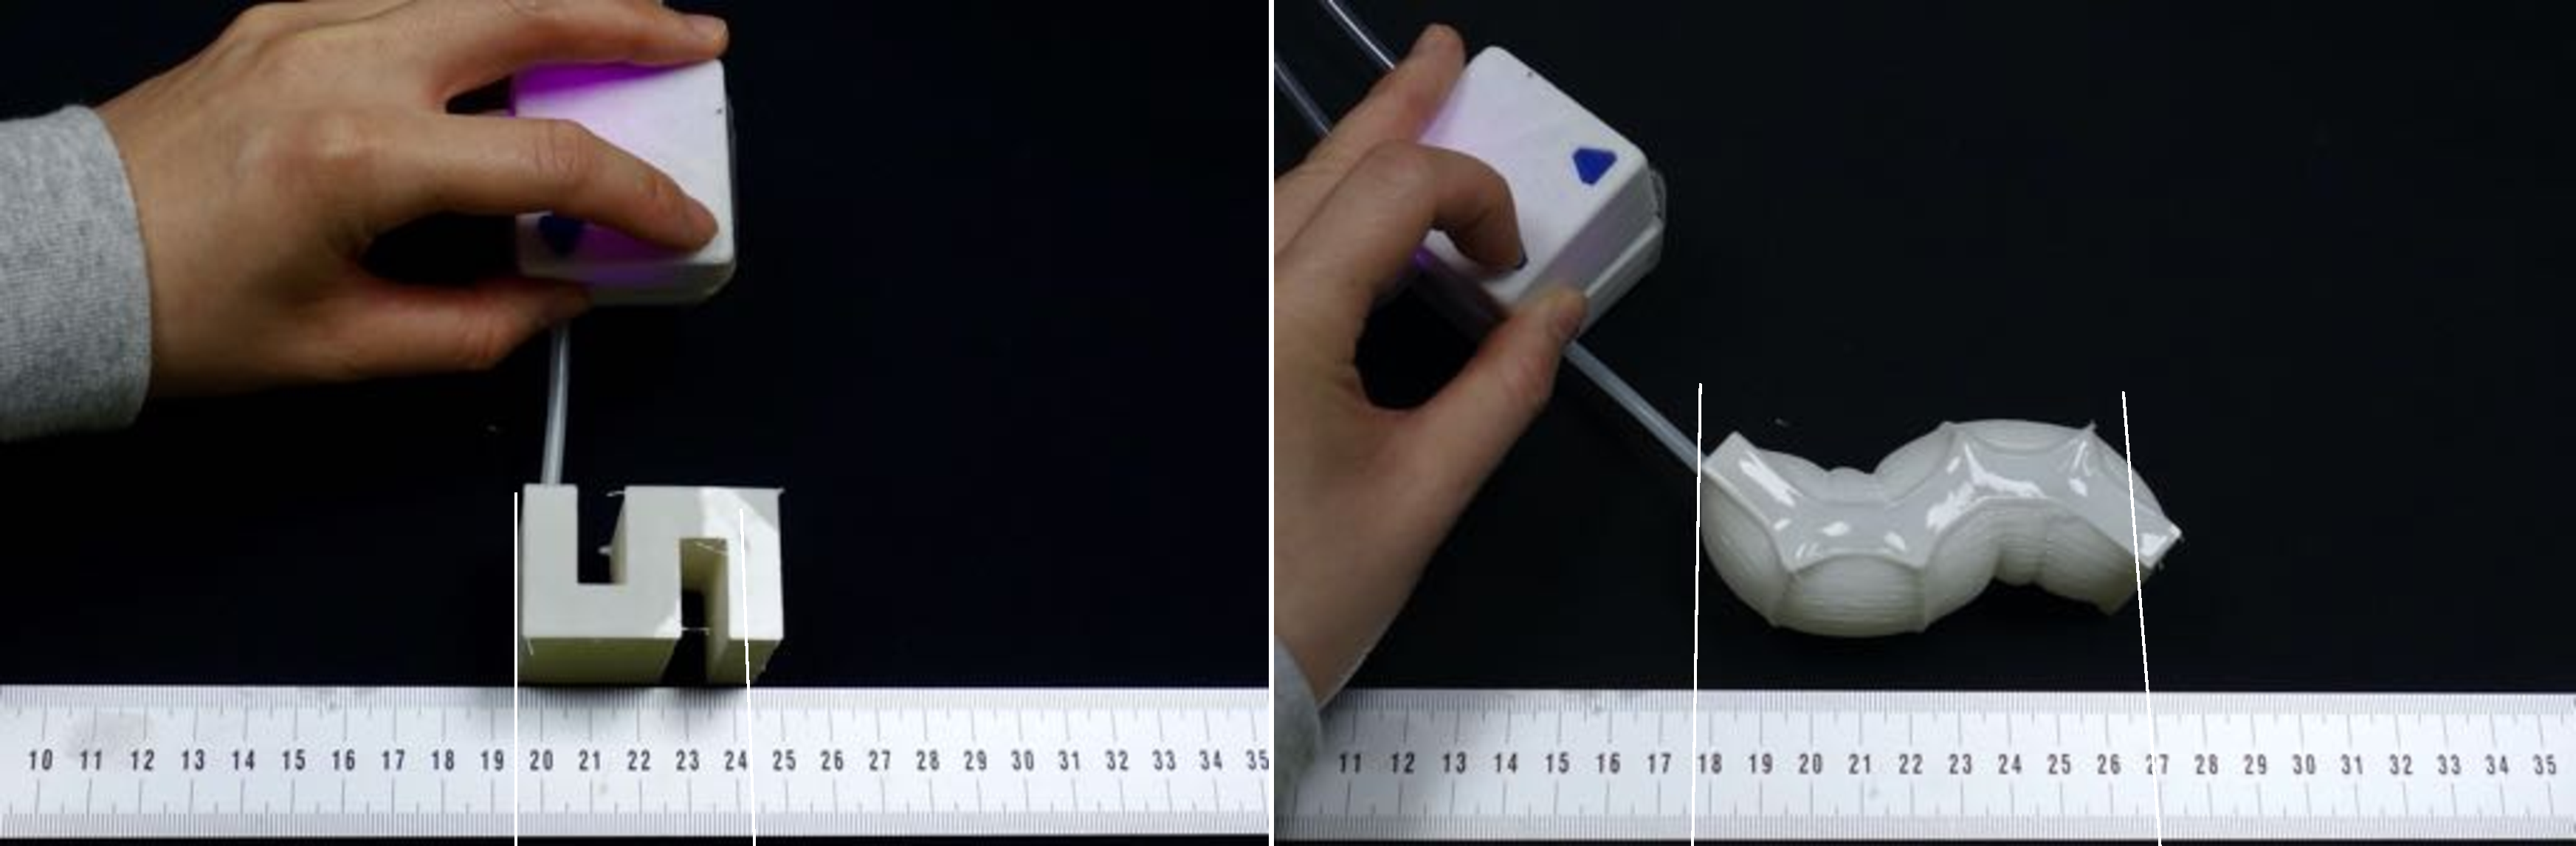
\includegraphics[width=0.45\textwidth]{print-and-play/morphees/Characterization_s.pdf}
        \caption{Our characterization setup. To measure the length change of the
          Fold widget, we placed a printed widget next to a ruler and measured the
          length of both deflated and inflated states.}
        \label{fig:widget-char}
      \end{figure}

      Figure \ref{fig:char-plot} presents the results of our explorations. We
      learned that the parameters that influence the area sections of the
      widgets that are perpendicular to the direction of the shape-change affect
      the most the behavior of the widgets, while the parameters that affect
      area sections parallel to the direction of the shape-change negate the
      shape-changing capabilities of our widgets. We believe this is because
      parameters that are parallel to the direction of shape-change restrict our
      widgets' movement when inflated, but parameters that are perpendicular to
      this movement do not, while at the same time increasing the structure's
      inflatable volume.
        
      \begin{figure*}[htb]
        \centering
        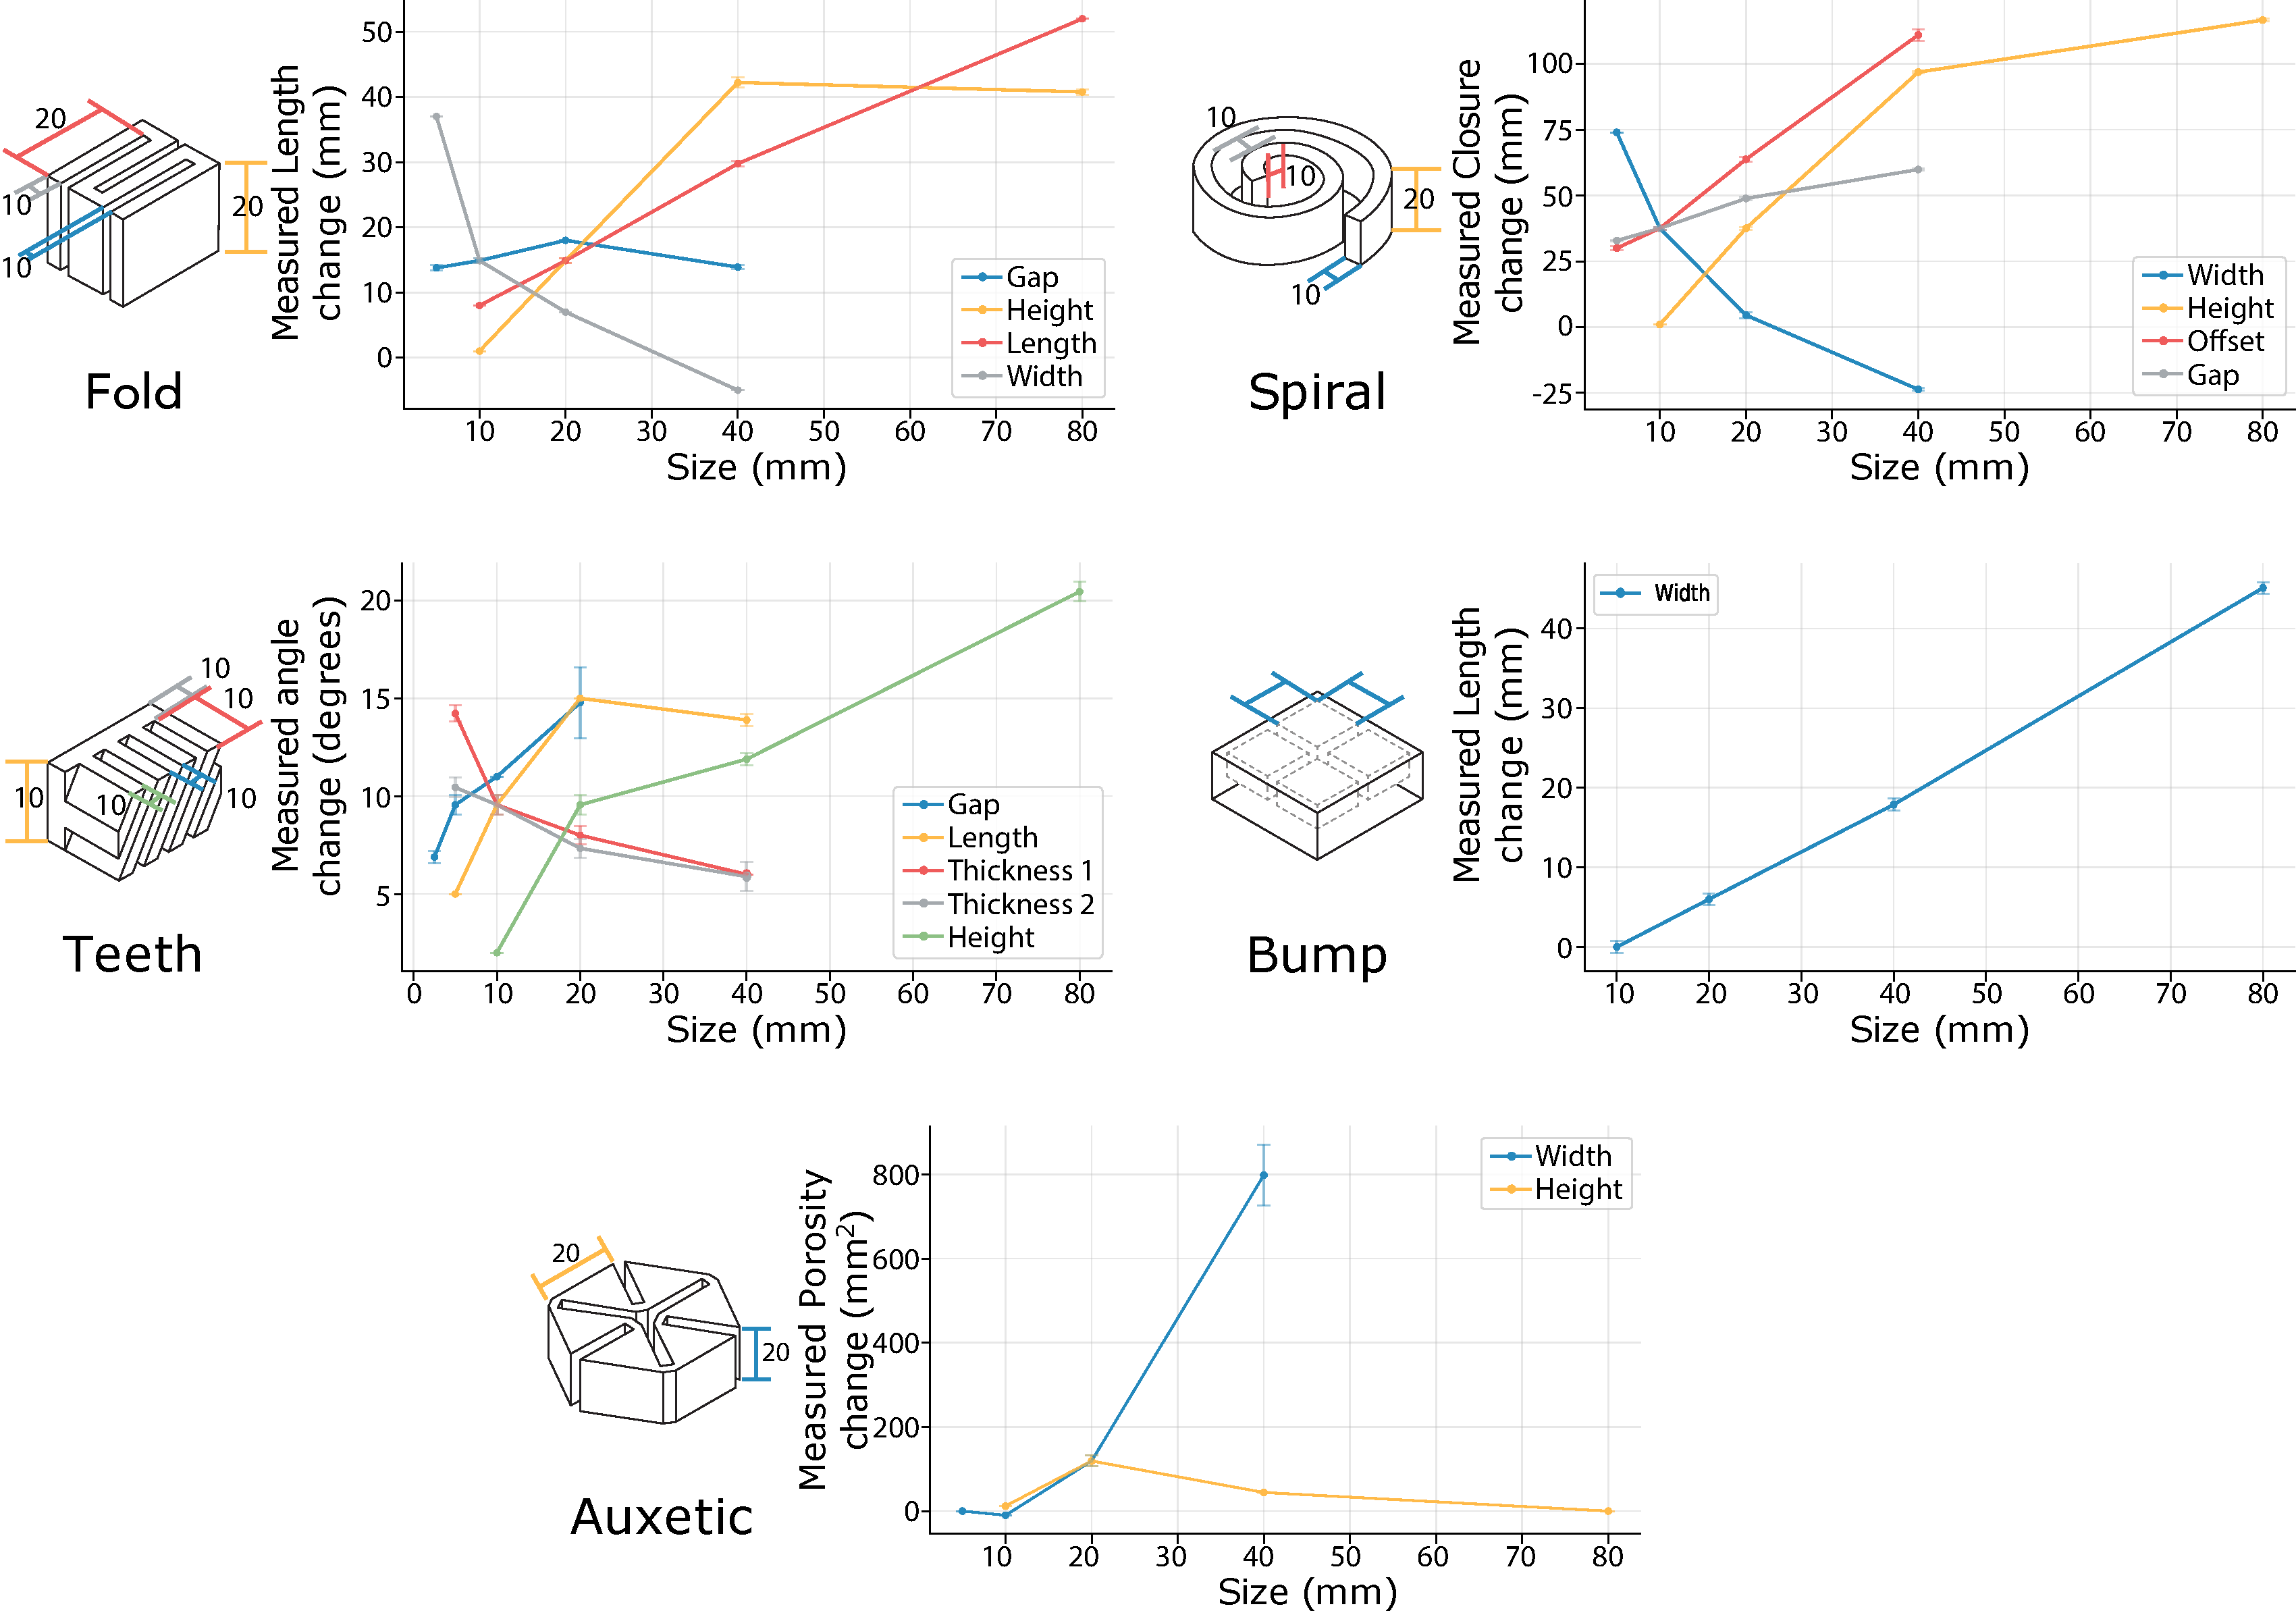
\includegraphics[width=1\textwidth]{print-and-play/morphees/chart v4.pdf}         
        \caption{Results of the characterization. These plots show magnitude of
          the modified features versus the change of shape the widgets expressed.
          The numbers on the widgets show the baseline size of the features. For
          example, Fold widget had a baseline parameters of gap 10 mm, length 20
          mm, height 20 mm, and width 10 mm. We then changed each parameter one by
          one, e.g., changed length from 10 mm to 80 mm (red line in the plot).}
        \label{fig:char-plot}
      \end{figure*}

    \subsection{Control Module}
      The final part of our toolkit is an electronic control module to allow
      designers to easily control the actuation of our widgets
      (Figure \ref{fig:module}). This module, measuring 4 cm x 4 cm x 4.5 cm,
      is made up of five components: (1) two electronic solenoid valves to
      control airflow to, and from the widgets; (2) a barometric pressure
      sensor; (3) a custom circuit board used to interconnect all the
      components from our module; (4) an LED to display to the designer the
      status of the valves; (5) and a micro-controller to drive all the
      components.  Once the widgets have finished printing, the designer
      proceeds to connect them to our control module.

      \begin{figure}
        \centering
        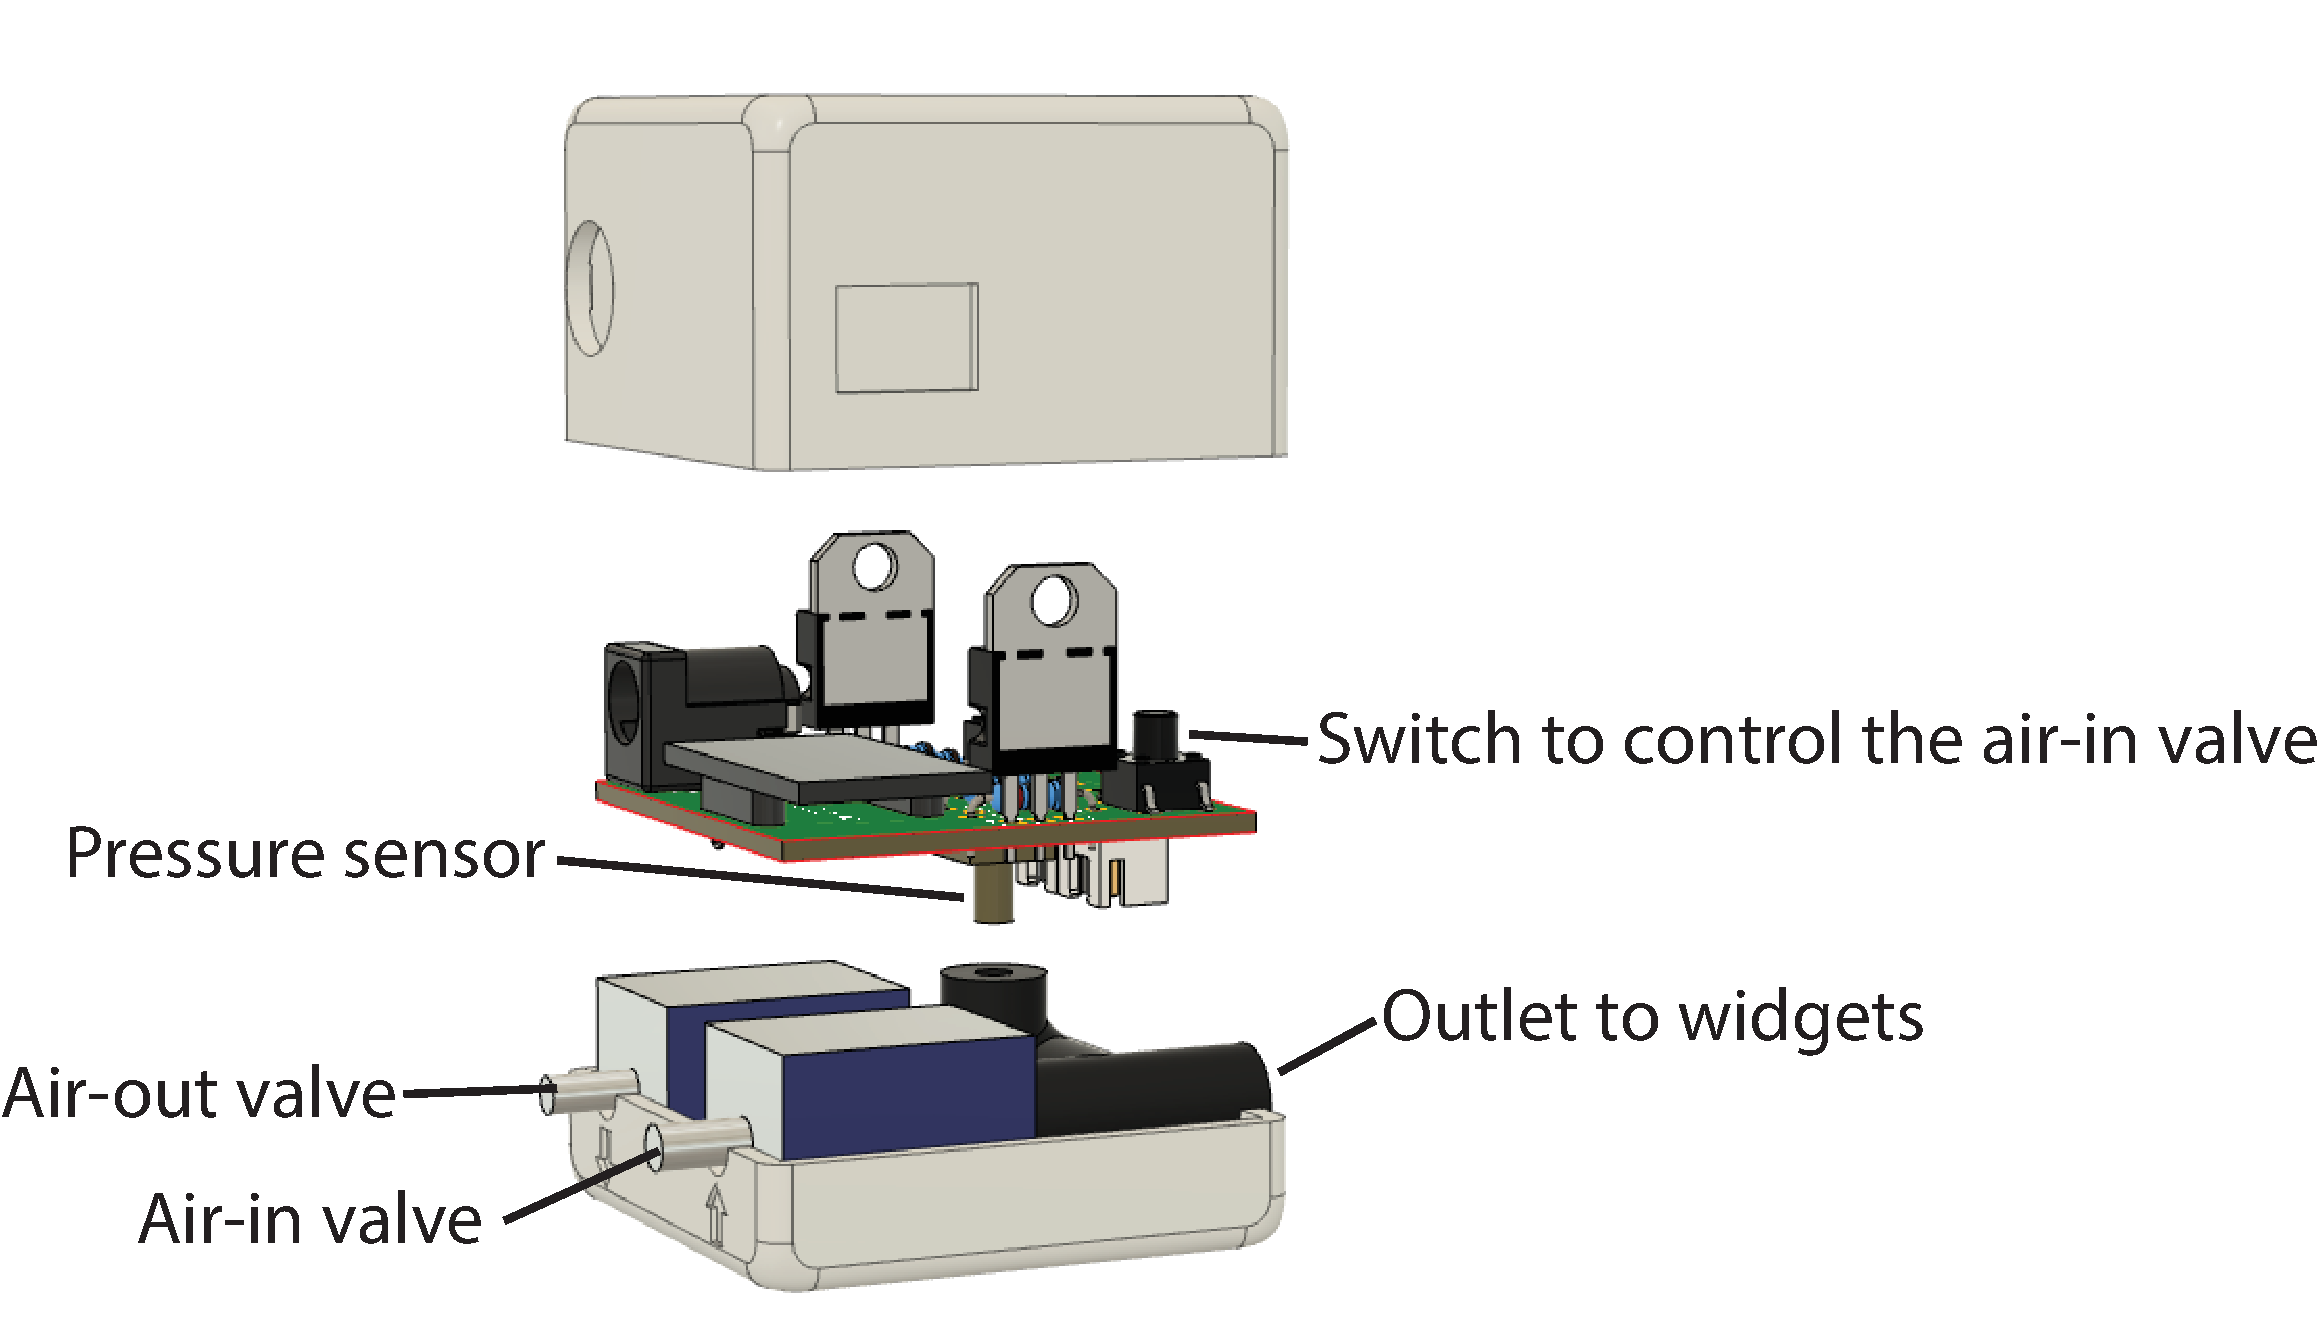
\includegraphics[width=0.4\textwidth]{print-and-play/morphees/Module_assemblyView.pdf}
        \caption{An exploded view of the control module. The module has two
          valves to let air in and out of the widgets.}
        \label{fig:module}
      \end{figure}

  \section{Demonstration}
    We present five applications to demonstrate the capability of \mp to express
    various shape-change features in different scales. These applications were
    created using our design environment, widgets, and modules, but were
    manually actuated by the authors.
     
    \subsection{Umbrella pusher}
      The umbrella pusher is to demonstrate the spiral widget's ability to hold
      an object.  It also uses the fact that widget's character that when it
      unbends less when is has a lower height (Figure \ref{fig:appl_umbrella}
      left). To create the umbrella pusher, we first created a spiral widget
      with 2cm height and three arcs with our plug-in. We then manually lowered
      the height of the central part to make the part hold an umbrella even when
      the widget is actuated. We then 3D printed the model with zero in-fill.
    
      The umbrella pusher can installed at an apartment entrance and hold an
      umbrella.  On rainy days, the spiral widget gets inflated and pushes the
      umbrella towards users when they approach to it
      (Figure \ref{fig:appl_umbrella} middle, right).
        
      \begin{figure}[htb]
        \centering
        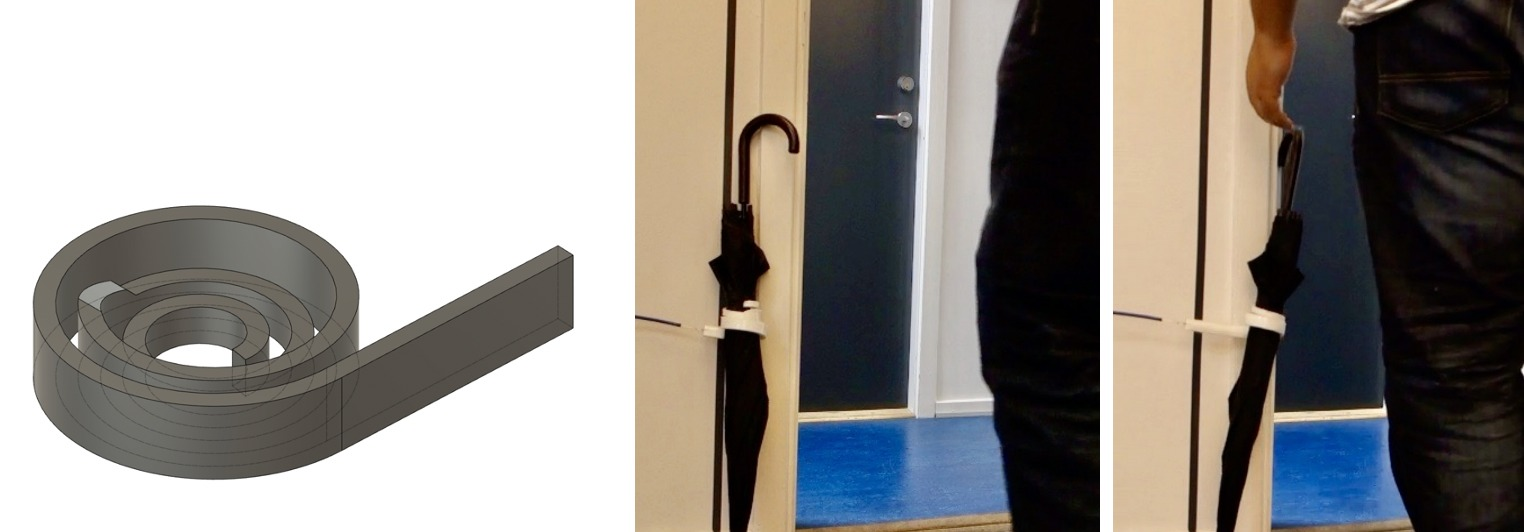
\includegraphics[height=3cm]{print-and-play/morphees/Fig_8.jpeg}
        \caption{Left: The 3D model of an umbrella pusher created by our plug-in
          and edited in CAD software. Middle: The umbrella pusher is holding an
          umbrella. Right: On a rainy day, the umbrella pusher slightly unbends
          and pushes the umbrella towards on the way of users to remind to take
          the umbrella. The central part of it unbends less and still holds the
          umbrella.}
        \label{fig:appl_umbrella}
      \end{figure}
   
    \subsection{Anti-rain phone case}
      The anti-rain phone case is to show that \mp supports heterogeneous
      shape-changes and integration with existing 3D models.  We combined three
      Teeth widgets and one Fold widget to create a shape that bends from back
      of a phone can elongate. We then combined them with a 3D model of a phone
      case form the Internet (Figure \ref{fig:appl_rainphone} left).  When the
      phone case is inflated, it bend over the phone screen and block rain,
      strong sun-light on the phone (Figure \ref{fig:appl_rainphone} middle,
      right). It can also prevent someone from looking at private information
      similarly to a shape-changing phone \cite{Roudaut:2013kz}.
        
      \begin{figure}[htb]
        \centering
        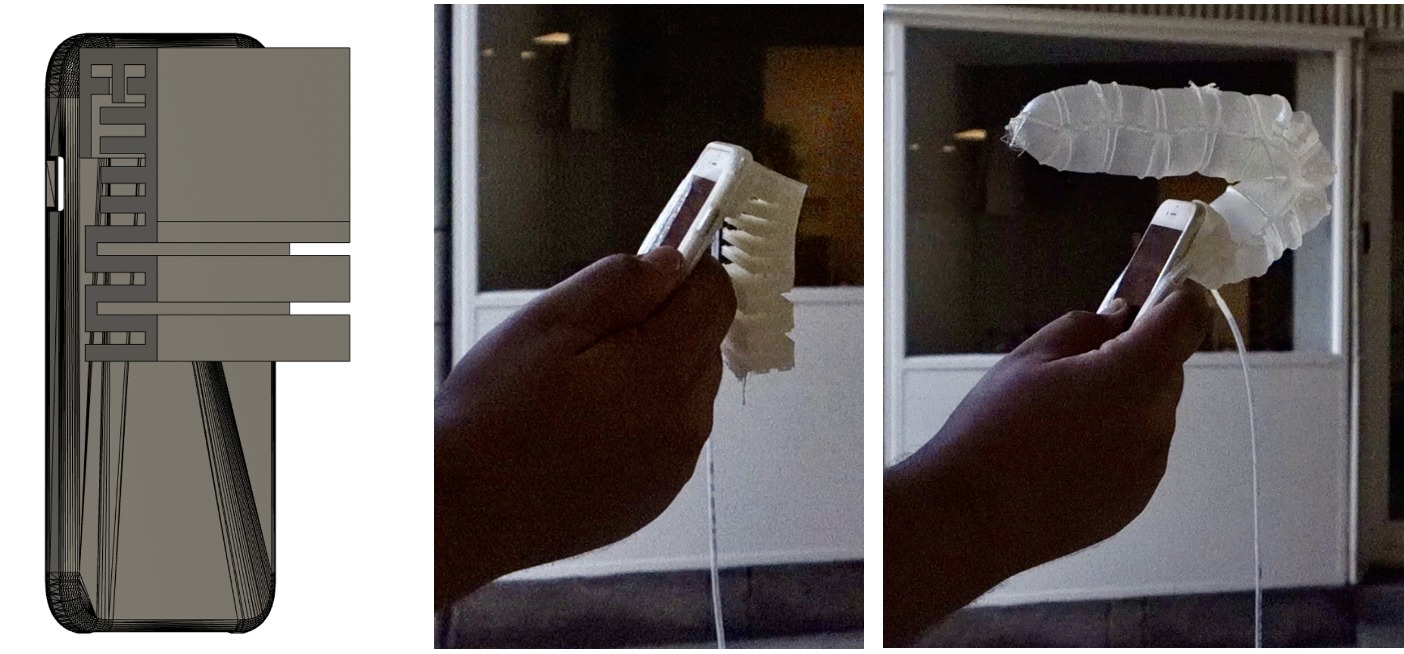
\includegraphics[height=4cm]{print-and-play/morphees/Fig_9.jpeg}
        \caption{Left: The 3D model of anti-rain phone case. Middle: A user
          holding a 3D printed anti-rain phone case. Right: When it rains, the
          phone case can inflate and block rain drops over the phone.}
        \label{fig:appl_rainphone}
      \end{figure}
    
    \subsection{Posture-correcting cushion}
      The posture-correcting cushion (Figure \ref{fig:appl_cushion}) is to show
      that \mp can handle high pressure and human weight.  We used the same 3x3
      Accordion widget from the characterization section.
      
      When users sit on the cushion in an incorrect posture, it can push them to
      remind them to sit correctly. Unfortunately, the pressure of the cushion
      was higher than the sensing range of the pressure sensors in the current
      version of our module.
      
      \begin{figure}[htb]
        \centering
        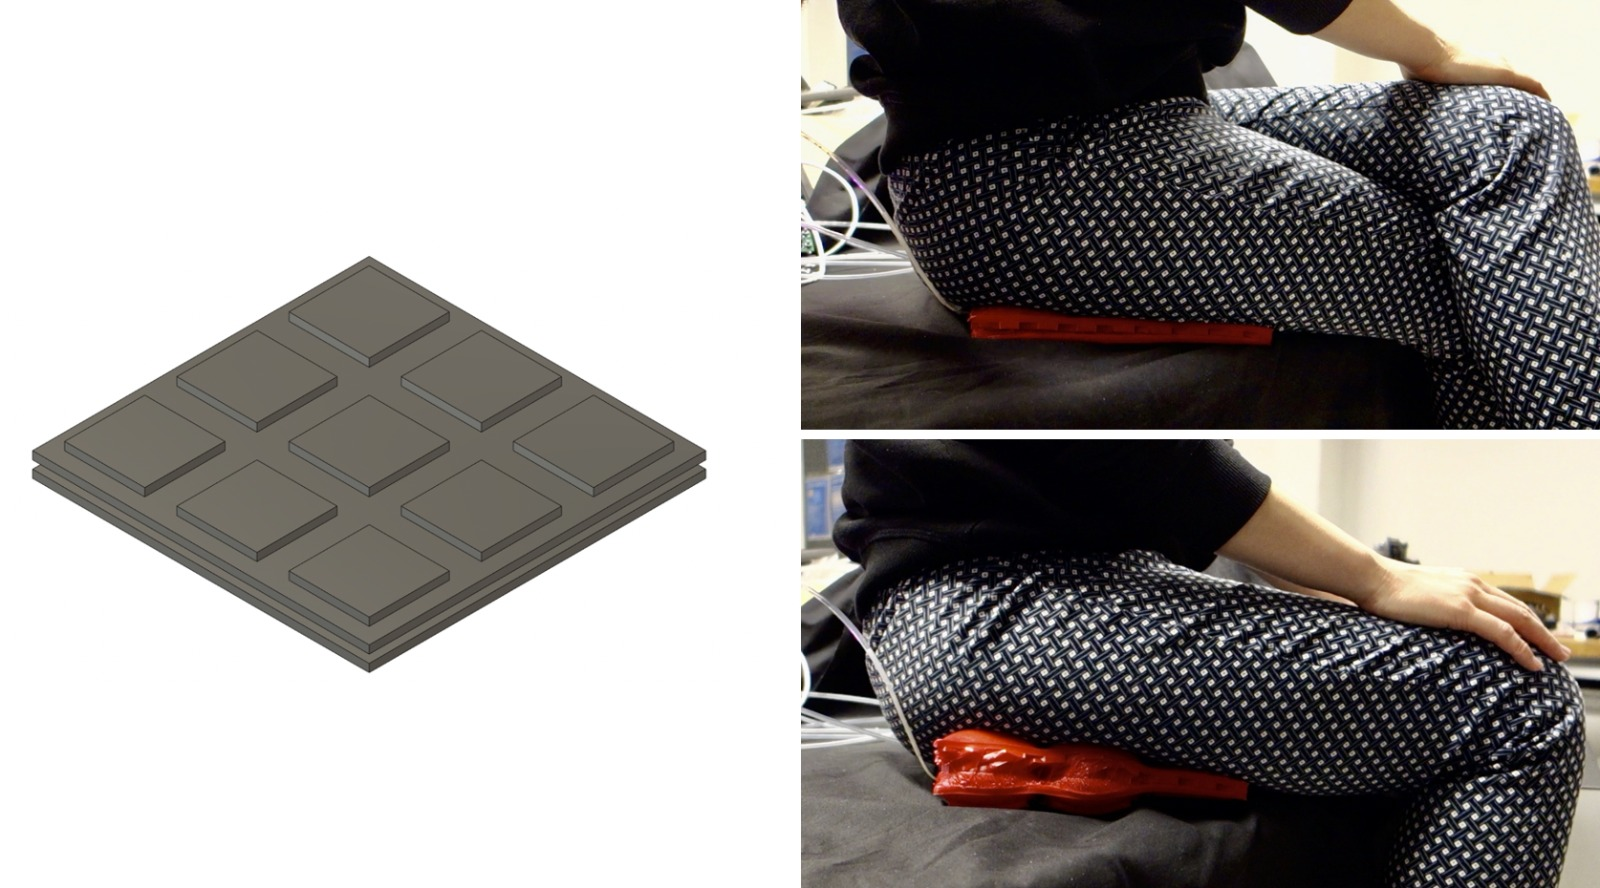
\includegraphics[height=4.7cm]{print-and-play/morphees/Fig_10.jpeg}
        \caption{Left: The 3D model of posture-correcting cushion. Middle: A
          user sits on the cushion learning forward. The cushion recognizes higher
          pressure at the front. Right: The front cushion inflates and correct the
          user's posture.}
        \label{fig:appl_cushion}
      \end{figure}
        
    \subsection{Physical bar chart}
      The physical bar chart (Figure \ref{fig:appl_barchart}) was specifically
      designed to replicate pin-based SCIs (e.g., \cite{10.1145/2501988.2502032,
      Nakagaki:2016jt, 7542185, 10.1145/2858036.2858316,
      10.1145/2702123.2702599}).  We wondered if \mp could easily replicate
      existing SCIs, and pin-based SCIs have been widely used to introduce novel
      interactions and understandings of SCIs.  Our 3D printer took 21 hours to
      print nine Fold widgets (~2.3 hr per widget), which would take longer than
      using off-the-shelf parts. However, the widgets would allow less assembly
      time because users just need to plug tubes to the widgets and connect them
      to modules.  Although it allowed quick prototyping, the final form is
      different from existing pin-based SCIs. First, they do not have the
      ``pin'' shape. To improve the form factor, users would need to print a
      static pin on top of each widget or assemble and hide the widgets. Second,
      the resolution is lower than high-resolution ones (e.g., a pin in inFORM
      \cite{10.1145/2501988.2502032} has a 9.525 mm$^2$ footprint). Currently a
      widget has a footprint of 625 mm$^2$ (2.5 cm x 2.5 cm) and need spaces
      between them. If we reduce the footprint of the widget, the widget would
      have less length change with the same number of folds. Additionally, we
      noticed the bar chart tilted slightly to one side when actuated. As a
      possible remedy, we could insert plastic separators between each of the
      fold widgets to prevent tilting on actuation.
        
      \begin{figure}[htb]
        \centering
        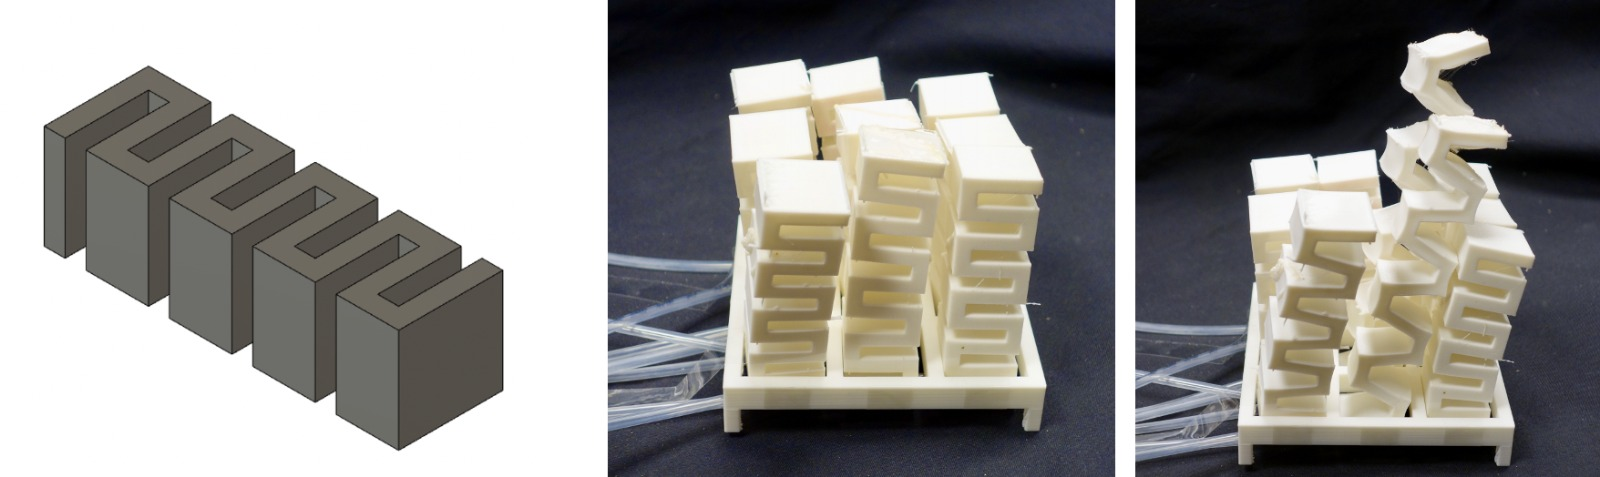
\includegraphics[height=2.5cm]{print-and-play/morphees/Fig_11.jpeg}
        \caption{Left: A 3D model of Fold widget. Middle: We 3D printed nine
          copies of the 3D model and put them in a grid. Right: Some of the
          widgets are actuated.}
        \label{fig:appl_barchart}
      \end{figure}
    
    \subsection{Window blind}
      The window blind is designed for an aesthetic purpose. We created seven
      Auxetic widgets in three different sizes, and then manually combined with
      added connecting space between the neighboring widgets
      (Figure \ref{fig:appl_windowblind} left). When inflated, the widgets
      expand and increase porosity between and within the widgets. User can
      adjust the porosity by changing the air pressure in the widgets.
        
      \begin{figure}[htb]
        \centering
        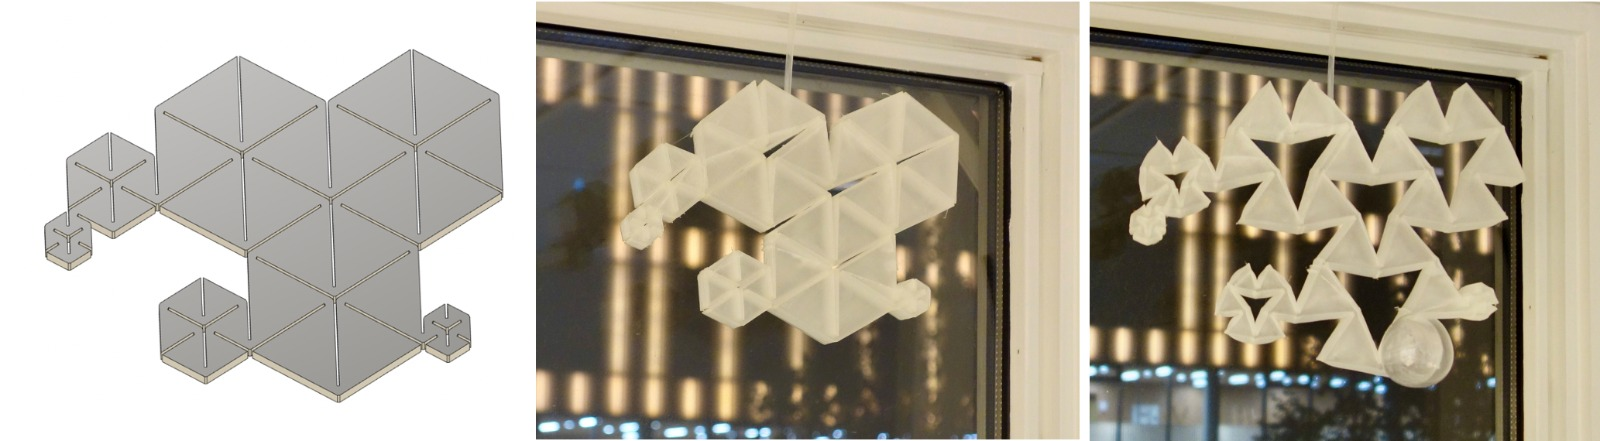
\includegraphics[height=2.4cm]{print-and-play/morphees/Fig_12.jpeg}
        \caption{Left: The 3D model of the window blind. Middle: Deflated window
          blind. Right: Inflated window blind.}
        \label{fig:appl_windowblind}
      \end{figure}
    
  \section{User Study}
    We conducted a user study to evaluate \mp plug-in. We were particularly
    interested if the plug-in meets the design rational we aimed.  As we aimed
    that our toolkit enables novices to create SCIs and also integrates with
    current practices, we invited both novice and expert users in our study, in
    terms of 3D modeling skills.
      
    \subsection{Participants}
      Participants were recruited through an advert on a social media page used
      by a local maker community and the word-of-mouth. Participants approached
      the researcher via email and we recruited 10 participants (age 25-64,
      female 2). 
        
      We got participants with both expert and novice skill levels in 3D
      modeling.  With novice users (P6-8,10, background in Computer Science,
      Communication, or Public Health. No or little 3D modeling experiences), we
      wanted to see if they can understand the toolkit and implement their ideas
      using our plug-in.  With experts (P1-7,9, background in Architecture,
      Industrial Design, or Robotics. Advanced skill in 3D modeling or using 3D
      modeling software at work), we wanted to see if the plug-in can integrate
      with their experience of 3D modeling and help them save time.  Four out of
      six expert participants had experience in Fusion 360 (P2,3,5,9).
      Regarding experiences related to SCIs, P9 was both a hobbyist and also
      founded a small-sized enterprises in soft robotics.  P4 had experiences in
      fabricating inflated tin foils, and P2 had experiences in compliant
      mechanisms \cite{howell2013compliant}.  We compensated each participant
      with a ~\$20 worth local product.
        
    \subsection{Procedure and Tasks}
      The studies were performed in person for all participants aside from P9,
      where the study was done via video conference. Each study took around one
      hour and was recorded via audio, video, and screen recording with consent.
        
      Each study consisted of three parts. First, the participants signed a
      consent form and answered to biographical questionnaire (10 min). Second,
      we showed examples of SCIs \cite{10.1145/2501988.2502032, Yao:2013bg}, and
      asked the participants to brainstorm ideas for new shape-changing
      interfaces they want (20 min). To help them brainstorm, we asked them to
      think about their work and daily life. We also provided them a few ideas
      from other participants when they wanted \cite{10.1145/2675133.2675239}.
      They were then asked to choose one of the ideas to design for the rest of
      the user study.  Lastly, we demonstrated our printed widgets and two
      example applications (umbrella pusher and anti-rain phone case) and asked
      the participants to 3D model their ideas using \mp plug-in in a
      think-aloud manner (30 min). We showed them how to use the plug-in and
      supported them when they do not know how to use other Fusion 360
      functions. After the 3D modeling, we asked them questions about strengths
      and weaknesses of the \mp plug-in. Note that the Auxetic widget was not
      implemented in the plug-in at the moment of the study.

    \subsection{Results}
      Three of the authors analyzed the transcribed interviews from all the
      participates. We specifically focused on the design rationale we discussed
      earlier in the paper. Additionally, we wanted to understand the usability
      of \mp plug-in and the potential direction for enhancing the plug-in.
          
      \subsubsection{General response}
        Overall, all participants were excited when seeing our widgets and
        example applications, showing both the potential novelty and usability
        of \mp for designing SCIs. P10 stated: ``It was relatively straight
        forward and intuitive... ''. P4 was enthusiastic in seeing all the
        widgets we developed and exploring their actuation. 
        
      \subsubsection{Reducing authoring time and complexity}
        All participants agreed that the authoring time and complexity of
        designing from scratch is reduced by our plug-in. All participants
        except P8 could closely design what they sketched using the plug-in.
        This demonstrates the potential for fast adoption of our toolkit plug-in
        for designing novel SCIs.  P3 emphasised that our plug-in ``... only
        required a little bit of modification to execute my idea.'' Similarly,
        P6 stated that they were ``positively surprised at how easy it was to
        implement a version of my sketch using the basic shapes available.''
        This positive response is likely due to our plug-in providing ready to
        use widgets, where users do not need to design from scratch.

        In terms of customisation, participants also stated that they would like
        to directly edit the widgets by dragging arrows (e.g., for stretching
        etc) and not only use numeric input for parameters when creating the
        widgets. Two participants also commented that they wanted to edit more
        parameters. For example, P3 wanted one and a half layers in Accordion
        and P4 also wanted to change the length of gap in Accordion, which is
        currently fixed to 1cm.         

        \subsubsection{Empowering new audiences}
          Complex 3D modeling can be a barrier for non-expert users who want to
          step in the area of SCIs. The four novice participants we recruited
          appreciated that our plug-in enabled them to create 3D models without
          expert skills required. The 3 out of 4 novices (P6, P7, P10) were able
          to understand the concept of SCIs, the actuation capabilities of our
          widgets, and design their own 3D model from their sketches.
          
        \subsubsection{Integrating with current practices and infrastructures}
          \mp aimed to use existing, consumer-level tools  to fabricate SCIs.
          To achieve this, we built the widget design software as a plug-in for
          Fusion 360.  Participants who had experiences with Fusion 360 showed
          efficiency of creating their intended designs. For example, P2 was
          able to create a relatively complex shape in less than 30 minutes (see
          Figure \ref{fig:p2}). They created Bump widgets and added rigid parts
          around them as a handle to hold a pen by squeezing one bump widget. 
          
          \begin{figure}
            \centering 
            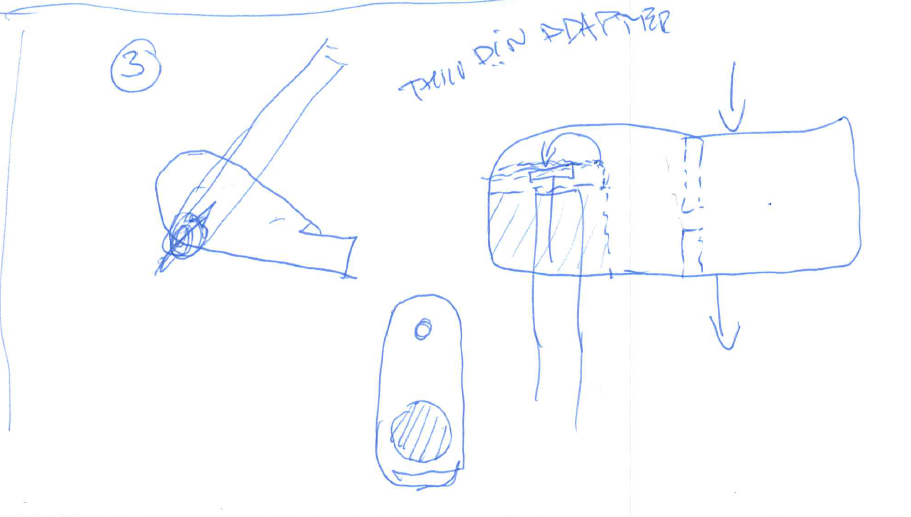
\includegraphics[height=3.5cm]{print-and-play/morphees/P2 draft.png} 
            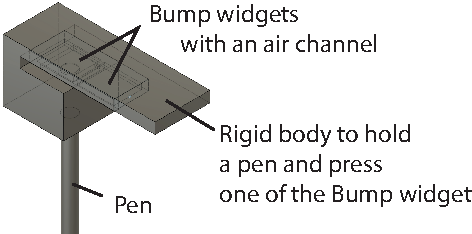
\includegraphics[height=3.5cm]{print-and-play/morphees/UserStudy_P2_3DModel.pdf}
            \caption{Idea sketch and its 3D model from P2. It is a pen-pressor
              to help people who lack fine motor skills. The two Bump widgets
              inside of the rigid body has an air channel between them. Users can
              press the rigid body to compress one of the widgets, and the air in
              the widget would travel to the other widget to press the top of the
              pen.}
            \label{fig:p2}
          \end{figure}
          
          On the other hand, users who were not used to 3D modeling or Fusion
          360 struggled with using functions other than the \mp plug-in.  They
          had to tell us what they want to do, and we had to tell them where the
          related functions are and how to use them. It hindered them from
          exploring and editing the 3D models. To make \mp widespread, we need
          to create plug-ins for other CAD software or develop an independent
          software.
                  
        \subsubsection{Enabling creative exploration}
          The plug-in enabled creative exploration by  letting users explore the
          widgets and their parameters.  As P3 explained: ``Another advantage
          would be to see that. You know, not all the time we can imagine all
          the possible shapes. When you have a plug-in, you see an idea where to
          start with, `Okay, this may be possible' ... Probably I can also do
          something with that...just by looking at the module I can learn what
          are the possibilities''.
                  
          However, the difficulty of editing the widgets caused difficulties for
          users (especially novices) to freely explore the widgets. More than
          one participant revealed the desire for characterization of widgets as
          well as real time simulation of shape-changes for better understanding
          how the widgets would behave. Another suggestion for improving the
          creativity was having random or irregular shapes automatically
          generated for users to explore the properties of shape changing
          widgets (P3).
      
  \section{Discussion and Future Work}
    \mp's widgets are able to express seven of the eleven shape-changing
    features detailed in the Morphees+ taxonomy~\cite{10.1145/3173574.3174193}.
    We intentionally focused on features of this space that resulted in
    significant physical change, what meant that features like granularity,
    stretchability, strength, and speed are not in the scope of this work. As
    mentioned earlier, we use a constant pressure of 100kPa to power our module
    and widgets, which causes smaller widgets to be actuated quicker than larger
    ones. Future work can explore how to employ pneumatic actuation to represent
    these features by using techniques such as jamming~\cite{Follmer:2012cx}, or
    by dynamically regulating pressure to vary actuation speed.
      
    Future work can also continue to explore the effects of different
    fabrication parameters on the shape-change potential for \mp widgets. For
    example, our Fold widget not only changes length when actuated, but also
    curvature as the surface becomes uneven and round. This effect is caused by
    the homogeneous thickness of the outer walls of the widgets. There is
    opportunity to explore the effects of such parameters to more precisely
    control how each widget expresses its respective shape-changing features.
      
    Conversely, while we were able to successfully fabricate shape-changing
    widgets using consumer-level elastic filament (Ninjaflex, shore 85A) on
    off-the-shelf hardware, the limited elasticity of this material reduced the
    shape-changing capability of our designs. For example, when we fabricated
    our Fold widget with 1~cm height, its shape varied very little when
    inflated. More elastic materials, such as silicone, could allow larger shape
    change on smaller objects, at the expense of ease of fabrication.
      
    Continuing, although our control module only presents a single air output to
    actuate the widgets, designers can actuate multiple widgets in tandem by
    making use of Y-splitters to connect multiple widgets to a single module.
    Additionally, while a single computer can control multiple modules, these
    must be connected via USB. We plan to explore different ways to control our
    modules (e.g., via Bluetooth, or WiFi), and alternatives for controlling
    various widgets with a single module. These improvements could benefit the
    portability of our work.
      
    Once printed, our widgets are airtight, and capable of holding their shape
    after actuation. While in our experiments we used a dedicated air compressor
    to power our module and widgets, in the future we wish to explore
    more-accessible options by testing the efficacy of miniature air pumps. A
    further benefit could be miniaturization by embedding pumps into the control
    module.
      
    Finally, we plan to evaluate \mp in terms of the quality of interaction. It
    would be interesting to compare \mp to SCIs that have other mechanism other
    than pneumatic actuation, such as mechanical \cite{10.1145/3173574.3173724}
    or manual \cite{10.1145/3131277.3132179}.% in VR. %don't give it away!
      
  \section{Conclusion}
    In this paper, we presented MorpheesPlug, a toolkit for prototyping
    shape-changing interfaces (SCIs). By providing six widgets and using
    pneumatic actuation, the toolkit expresses seven shape-change features. To
    make the widgets accessible to users, we implemented a plug-in for CAD
    software where users can change the parameters of the widgets. We presented
    three applications using MorpheesPlug and conducted user studies to
    illustrate MorpheesPlug's ability to express shape-change features and
    easily prototype SCIs.  We envision that MorpheesPlug can be a first step
    towards building a standardized toolkit for prototyping SCIs.